\documentclass{bioinfo}
\usepackage{natbib}
\usepackage{url}
\copyrightyear{2009}
\pubyear{2009}

\newcommand{\Rpackage}[1]{`\texttt{#1}'}
\newcommand{\Rclass}[1]{\textsl{#1}}
\newcommand{\subfig}[1]{\textbf{#1}}

\begin{document}
\firstpage{1}

\title[Modular analysis]{Modular analysis of gene expression data with R}
\author[G\'abor Cs\'ardi \textit{et~al}]{G\'abor Cs\'ardi\,,$^{1,2}$,
  Zolt\'an Kutalik\,$^{1,2}$ and Sven Bergmann\,$^{1,2}$}
\address{$^{1}$Department of Medical Genetics, and
  $^{2}$Swiss Institute of Bioinformatics,
  University of Lausanne, Rue de Bugnon 27, CH-1005 Lausanne,
  Switzerland.}

\history{Received on XXXXX; revised on XXXXX; accepted on XXXXX}

\editor{Associate Editor: XXXXXXX}

\maketitle

\begin{abstract}
\section{Summary:}
Large sets of data, like expression profiles from many samples, require
analytic tools to reduce their complexity. The Iterative Signature
Algorithm (ISA) is a biclustering algorithm. 
It was designed to decompose a large set of data into so-called
``modules''. In the context of gene expression data these modules consist of
subsets of genes that exhibit a coherent expression profile only over a
subset of microarray experiments. Genes and arrays may be attributed to
multiple modules and the level of required coherence can be varied resulting
in different ``resolutions'' of the modular mapping. 

In this short note, we introduce two BioConductor \citep{BioC} software
packages written in GNU~R: The~\Rpackage{isa2} package includes an optimized
implementation of the ISA and the~\Rpackage{eisa} package provides a
convenient interface 
to run the ISA, visualize its output and put the biclusters into
biological context. Potential users of these packages are all R and
BioConductor users dealing with tabular (e.g. gene expression) data.

\section{Availability:}
\href{http://www.unil.ch/cbg/ISA}%
{\url{http://www.unil.ch/cbg/ISA}}
\section{Contact:} \href{Sven.Bergmann@unil.ch}{Sven.Bergmann@unil.ch}
\end{abstract}

\vspace{-0.7cm}
\section{Introduction}

% How the ISA works
The ISA can be applied to identify coherent substructures (i.e. modules)
from any rectangular matrix of data. To be specific we consider here the
case of transcriptomics data corresponding to a set of gene-expression
profiles from a collection of samples. The method has been described in
detail in Refs~\citep{isamod,isa}. Here we only give a brief summary.

The ISA identifies modules by an iterative procedure. The algorithm starts
from an input seed (corresponding to some set of genes or samples) which is
refined at each iteration by adding and/or removing genes and/or samples
until the process converges to a stable set, which is referred to as a
transcription module.

The output of ISA is a collection of potentially overlapping
modules. Every module contains genes, that are over- and/or
under-expressed, in samples that belong to the module.
In every module, each gene and each sample is attributed a
score between minus one and one, that reflects the strength of the
association with the module. Moreover, if the scores of two genes of a
module have the same sign, then they are correlated (across the
samples of the module), opposite signs mean
anti-correlation. Similarly, if two sample
scores have the same sign, then these samples are correlated (across
the genes of the module), opposite signs indicate anti-correlation.

For other biclustering algorithms, please see e.g.
\citet{cheng00,getz00,califano00,sharan02,tanay04,barkow06} and
\citet{ihmels04} for a review.

\section{Methods}%
\label{sec:methods}

\begin{figure*}
\centering
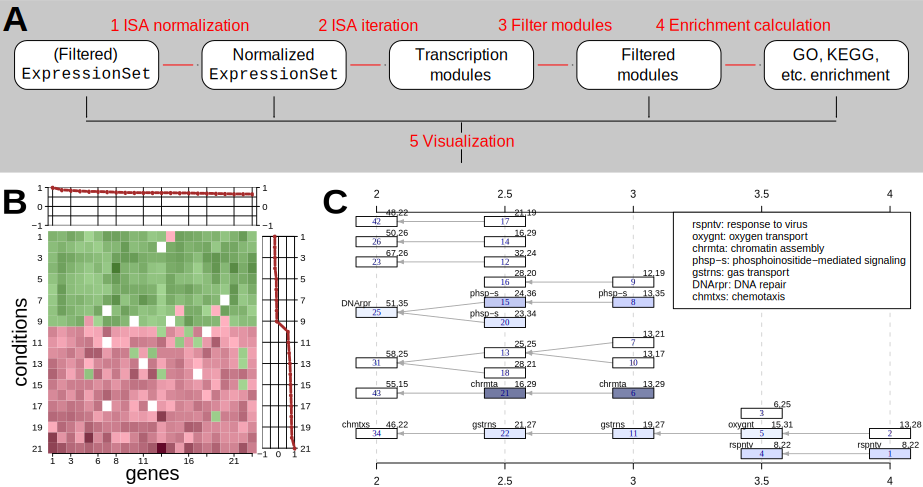
\includegraphics[width=0.842\textwidth]{isa2workflow3}
\caption{\subfig{(A)} Work flow of a typical modular analysis with the
  \Rpackage{eisa} package. See text for details.
  Subfigures \subfig{B} and \subfig{C} were generated
  using the acute lymphoblastic leukemia data set, see
  \citep{chiaretti04} and the \Rpackage{ALL} R package.
  \subfig{(B)} Heatmap for a single module, showing coherent
  expression of the genes across the samples. The red lines are the gene and
  sample scores.
  \subfig{(C)} Module tree. Each rectangle is a module; its numeric id
  is shown on top of it. See the definition of the edges in the
  text. Modules are colored 
  according to their Gene Ontology enrichment $p$-values, the codes of
  the enriched GO categories are shown in the top-left corner of the
  rectangles. The top-right corner shows the number of genes and
  conditions in the module. The gene thresholds used for finding
  the modules is shown on the horizontal axes.
}
\label{fig:workflow}
\end{figure*}

A typical modular analysis for gene expression data includes the following
steps:

% Batch correction
\emph{Batch correction.}
To study the global organization of a transcription program including
many aspects of transcriptional regulation one often combines several
microarray experiments into a single dataset. In such a case
additional data normalization is crucial to reduce the bias due to
the constituent datasets. Several methods address this challenge,
see e.g.~\citep{johnson07} for an algorithm that has a GNU R
implementation.

% Filtering
\emph{Gene filtering.}
Genes that have very low expression levels in all samples, carry little if
any information and may reflect ineffective array probes, etc. Since these
genes are likely to contribute mostly noise to the
analysis~\citep{hackstadt09}, we suggest removing them before running
the module identification of the ISA.

% Normalization.
\emph{ISA normalization.} (Step 1 in Fig.~\ref{fig:workflow}.)
In each iteration the ISA computes thresholded weighted sums of expression
levels over either genes or samples. Since different genes 
typically show different levels of base
expression and variance, it is important to standardize expression
levels to $Z$-scores. The ISA uses two sets of $Z$-scores, one
calculated for each gene across all samples, the other for each sample
across all genes.

% Random and smart seeding.
\emph{Random and smart seeding, ISA iteration} (Step 2.)
The iterative procedure of the module identification is typically applied to a
large number of seeds. In the unsupervised approach these seeds are chosen
randomly to sample uniformly the immense search space. We also implemented a
semi-supervised method, to which we refer as ``smart seeding'', where the
seeds are biased to start with certain sets of genes or samples based on
prior knowledge. The ISA can be performed with random or smart
seeds, depending on the application.

% Merging the modules.
\emph{Merging and filtering the modules.} (Step 3.)
It is possible that several seeds converge to the same, or very similar
biclusters. This step eliminates such duplicates.
To access the significance of a module, we designed a robustness
measure, that can be used to filter out spurious modules. This is done
by applying the ISA to scrambled input data in order to obtain a
reference (null) distribution for the significance scores.

% Module trees.
\emph{Module trees.}
The ISA works with two stringency threshold parameters, the gene
threshold and the sample threshold. ISA modules can be organized into
a directed graph, to which we refer as ``module tree''. An edge from module
$A$ to module $B$ indicates that the ISA converges to module $B$ from module $A$,
with the same threshold parameters that were used to find module
$B$. A module tree provides a hierarchical modular description of a
dataset.

\section{Implementation}%
\label{sec:implementation}

The ISA and accompanying visualization tools are implemented in two R
packages. The \Rpackage{isa2} package contains the implementation of
the basic ISA itself; this package can be used to analyze any tabular
data. The \Rpackage{eisa} package builds on \Rpackage{isa2}. It adds
support to standard BioConductor data structures; and
contains gene expression specific visualization tools (see
Fig.~\ref{fig:workflow} for examples).

Both the \Rpackage{isa2} and \Rpackage{eisa} packages support two
workflows. The \emph{simple workflow} involves a single R function
call and runs all ISA steps (1-3 in Fig.~\ref{fig:workflow}) with
their default parameters.

In the \emph{detailed workflow} every step of the modular analysis 
is executed separately, possibly with non-default parameters. This allows
the users to tailor the ISA according their needs.

% \subsubsection{Visualization}

The \Rpackage{eisa} package implements a set of visualization
techniques for modules (see Fig.~\ref{fig:workflow} for examples).

The \Rpackage{biclust} package, \citep{biclust}, implements a number of
biclustering algorithms in a unified framework. The \Rpackage{eisa}
package include tools to convert between \Rpackage{biclust} and ISA
biclusters. This allows the cross-talk of the functions in the two
packages.

Additional information and a Matlab implementation of ISA are
available on the ISA homepage. 

\vspace*{-0.5cm}
\section*{Acknowledgement}

\paragraph{Funding\textcolon} The authors are grateful to the Swiss
Institute of Bioinformatics, the Swiss National Science Foundation
(3100AO-116323/1), and the European Framework Project 6 (through
the EuroDia and AnEuploidy projects).
\paragraph{Conflict of interest\textcolon} None declared.

\bibliographystyle{natbib}
\bibliography{isa}

\end{document}
